\documentclass{beamer}
%Antibes a bande
%Bergen hipster
%Goettingen clean
%Marburg
\usetheme[watermark=polito-mark]{Torino}
\title{A framework for automated\\object detection and gripping}

\author{Simone Baratta}
\institute{Dipartimento di Automatica e Informatica\\Politecnico di Torino}
\titlegraphic{
  \begin{columns}[T]
    \column{.3\textwidth}
    \begin{flushright}
    \center \includegraphics[height=0.75cm]{logo-comau} 
    \end{flushright}
    \column{.3\textwidth}
    \center \includegraphics[height=1.5cm]{logo-polito} 
    \column{.3\textwidth}
    \begin{flushleft}
    \vspace{0.1525cm}
    \center \includegraphics[height=0.4cm]{logo-isaac} 
    \end{flushleft}
  \end{columns}
}
\date{December, 2015}
\begin{document}
  \watermarkoff
  \begin{frame}
    \titlepage
  \end{frame}
  \watermarkon
  \section{Introduction}
  \subsection{Motivation of the project}
  \begin{frame}
    \frametitle{Why gripping?}
    Automation of tasks has played an important role for humanity
    since the industrial revolution, but..

    \pause
    Special-purpose, monholitical robots machines are \emph{not}
    cost-effective, and do \emph{not} solve all problems!
    
    \pause
    Teaching a robot how to manipulate perfectly common
    items would have many application fields, and lead enormous
    benefits to the industry
  \end{frame}
  \begin{frame}
    \frametitle{State-of-the-art autonomous manipulators}
    \framesubtitle{An overview}
    Many solutions have been developed into the industry to solve this 
    task effectively, and some are reaching the market:

    \alt<1>{
    \begin{columns}[c]
      \column{.4\textwidth}
      \center \includegraphics[height=0.8in]{pisa}
      \column{.6\textwidth}
         Pisa/IIT's SoftHand is able to grasp many objects by
          emulating the human structure
    \end{columns}}
    {\begin{columns}[c]
      \column{.4\textwidth}
      \center \includegraphics[height=0.5in]{versaball}
        \column{.6\textwidth} Empire Robotics' \emph{Versaball} uses a sphere to
        envelop the object and grasp it by aspiration
    \end{columns}}
    \visible<3>{

    Solutions for many of the robotics problems do exists, but:
    \begin{itemize}
      \item{Each available library specializes in completing a single
        task: \alert{do one thing, do it well}}
      \item{Heavy fragmentation $\rightarrow$ no standard way of thinking $\rightarrow$ difficult interoperability}
    \end{itemize}
    }
  \end{frame}
  \subsection{Problem statement \& expected results}
  \begin{frame}
    \frametitle{Goal of this project}
    Building a framework that can exploit state-of-the-art software
    and integrate it into a coherent abstraction layer, \emph{plus}
    providing it with a working, complete
    solution for grasping common objects
    \begin{itemize}
      \item{\emph{Modularity} is the key requirement for the whole framework}
    \end{itemize}
  \end{frame}

  \begin{frame}
    \frametitle{Amazon Picking Challenge}
    Big companies like Amazon \emph{need} to push the research on
    these topics in order to bring full automatization to their
    warehouses

    Amazon started this challenge at the 2015 edition of International
    Conference on Robotics and Automation (ICRA)

    Main requirements:
    \begin{itemize}
    \item{Concurrent robots must find and take requested objects from a shelf}
    \item{Robots must be \emph{fully autonomous} in their operation}
    \item{Extreme care must be taken not to damage other objects or
      take the wrong ones}
    \end{itemize}
  \end{frame}

  \section{Framework structure's overview}
  \begin{frame}
    \frametitle{Presentation overview}
    \tableofcontents
  \end{frame}
  \begin{frame}
    \frametitle{Presentation overview}
    \tableofcontents[currentsection]
  \end{frame}
  \subsection{Main modules' diagram}
  \begin{frame}
    \frametitle{Code structure}
    \begin{columns}
      \column{.5\textwidth}
      \center 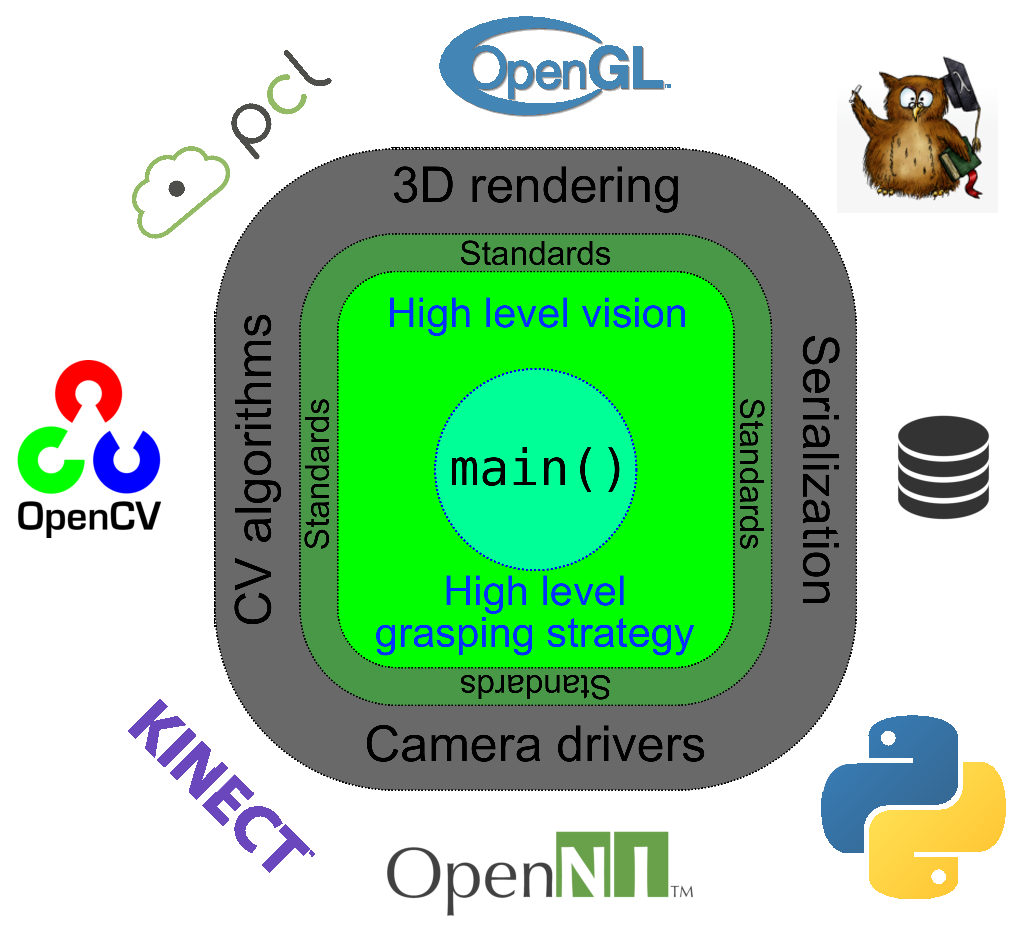
\includegraphics[height=2in]{structure}
      \column{.5\textwidth}
    \begin{overlayarea}{\linewidth}{12\baselineskip}
    \begin{itemize}
    \only<1>{\item{\texttt{main} of application is \emph{very tiny}, and leans
      against a set of abstracted modules which let it complete very
      high level tasks}
      \begin{itemize}
      \item{e.g.:}
        \begin{itemize}
        \item ``Grab a frame from here'';
        \item ``Find these objects into this image'';
        \item{``Tell me how to grasp
        one \texttt{kong\_duck\_dog\_toy} object from the objects
        you just found'';}
        \end{itemize}
      \end{itemize}
      }
    \only<2>{\item{Each module is \emph{totally independent} from
      the others -- you only have to follow standard conventions when
      interfacing other modules.}
      \begin{itemize}
      \item{Base modules developed for solving the APC: \emph{26}
        standalone shared libraries!}
      \end{itemize}
      \item{Modularity brings flexibility:}
      \begin{itemize}
        \item{Don't you like the default way of constraining grasp poses?
          You change it \emph{without need of touching other modules}!}
      \end{itemize}
    }
    \end{itemize}
    \end{overlayarea}
    \end{columns}
  \end{frame}

  \section{Main modules' description}
  \begin{frame}
    \frametitle{Presentation overview}
    \tableofcontents[currentsection]
  \end{frame}
  \subsection{Vision module}
  \begin{frame}
    \frametitle{Vision system}
    Each object is associated with a recognition algorithm, which is
    chosen by the programmer.

    Default recognition pipeline:
    \begin{itemize}
    \item{Is based on template matching on rigid objects;}
    \item{Makes use of the excellent Line-MOD algorithm, which is
      the current state of the art in its category;}
    \item{Provides accurate (\textless 1mm) pose estimation for each
      recognized object, which is \emph{fundamental} for the
      consecutive grasping stage.}
    \end{itemize}
  \end{frame}
  \begin{frame}
    \frametitle{Why template matching?}
    Template matching: learning a \emph{big} set of views for each object, then
    matching each view onto the scene to find the objects.

    \begin{itemize}
    \item{Big databases (30-100MB/object raw, 2-10MB/object
      compressed) are not a problem anymore;}
    \item{Additional informations (e.g. pose of the seen object) can
      be stored together with the template;}
    \item{Searching for multiple objects into an image has little
      added cost w.r.t. searching for only one.}      
    \end{itemize}
  \end{frame}
  \begin{frame}
    \frametitle{Template matching disadvantages}
    \alert{Main disadvantages of template matching:}
    \begin{itemize}
      \item{Steep recognition rate/performance tradeoff: matching many
      templates is slow;}
      \item{Long training stage: a lot (few \emph{thousands} per object!)
        of views are needed.}
    \end{itemize}
    \pause
      \color{green}{The proposed pipeline wants to solve these two problems:}
    \begin{overlayarea}{\linewidth}{5\baselineskip}
      \alt<+>{
      \begin{itemize}
        \item{Line-MOD algorithm was developed with speed in
          mind}
        \begin{itemize}
          \item{30fps on thousands of templates;}
          \item{Pyramidal matching for faster response;}
          \item{Innovative binary encoding of templates for reduced
            algorithm's size;}
          \item{Optimized algorithm to exploit modern CPUs' caches.}
        \end{itemize}
        \pause
      \end{itemize}
      }{
        \begin{itemize}
        \item{Automated training has been developed into the framework,
          which generates templates from CAD models.}
        \end{itemize}
      }
    \end{overlayarea}
    \end{frame}
  \begin{frame}
    \frametitle{Complete recognition pipeline}
    \begin{columns}
      \column{.3\textwidth}
      \includegraphics[width=\textwidth]{kinect}

      \visible<4->{\alt<4>{\includegraphics[width=\textwidth]{kinectsbagliacerchio}}{\includegraphics[width=\textwidth]{kinectnonsbagliacerchio}}}

      \column{.6\textwidth}

    Input for recognition comes from the Camera module, which provides
    colour+depth images, then\dots

    \begin{itemize}
      \pause
      \item{Recognition module asks Line-MOD to find some objects into
      the scene using their ID;}
      \pause
      \item{Line-MOD loads all the possible templates and returns a
        list of matches;}
      \pause
      \item{Line-MOD's thresholds kept low by design $\rightarrow$ \color{red}{\emph{absolute need for false positive's filtering}}!}
        \pause
        \begin{itemize}
        \item{First filter based on image's hue value;}
          \item{3D reconstruction and alignment: \color{green}{\emph{accurate pose estimation for free}}.}
        \end{itemize}
    \end{itemize} 
    \end{columns}
  \end{frame}

  \subsection{Gripping strategy module}
  \begin{frame}
    \frametitle{Gripping module: overview}
    \center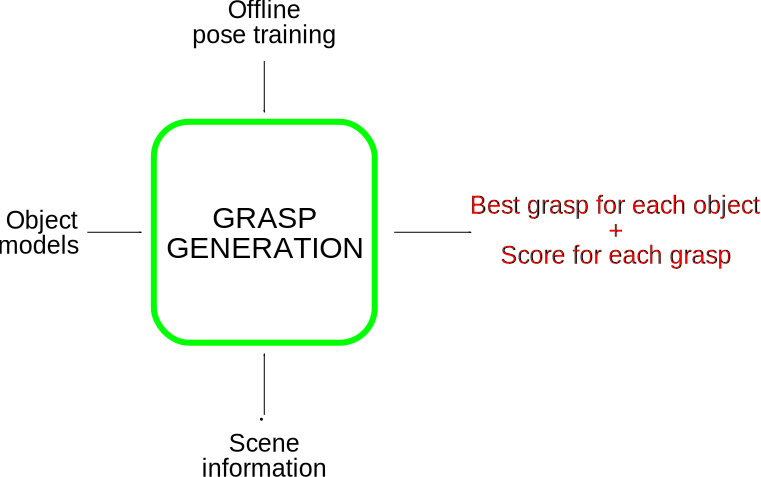
\includegraphics[height=2in]{grasp}
  \end{frame}
  \begin{frame}
    \frametitle{Object models for gripping}
    Main concepts used by the gripper are:
    \begin{itemize}
    \item{Object representation based on (composition of) elementary
      shapes;}
    \item{Each shape knows its representation at different abstraction levels (equation,
      surface, points);}
    \item{Access to objects' structure is done transparently
      through class polymorphism;}
    \end{itemize}

    \pause
    Grasp poses classified by a ``score function'' which
      represents the probability of hitting other objects during
      manipulation:

      \alert{Gripper is ``intersected'' with the scene, and the
        volume of the intersection is used to compute the
        ``badness'' of a pose.}
  \end{frame}

  \begin{frame}
    \frametitle{Pose training}
    Poses are given by sets of poses stored into a file.
    
    Grasping poses can be generated in multiple ways:
    \begin{itemize}
    \item{Automatic generation from geometrical info (e.g. ``all
      points on this plane are good'';}
    \item{Custom grasps can be added by hand.}
    \end{itemize}
      
    Preference scores assigned to each pose: ``this pose is good, but
    only if this other pose is not acceptable''.
    
    \pause
    
   \alert{Each grasp only sets the \emph{minimum} constraints on the pose:
    the others are fitted automagically in order to give the gripper
    its most natural pose.}
  \end{frame}

  \begin{frame}
    \frametitle{Best pose search}
    Computation of intersections is done on two levels to maximize
    performance:
    \begin{itemize}
    \item{Slow, always working algorithm based on shapes' approximation
      using small cubes;}
    \item{Heuristic database which has precedence when a faster
      algorithm is known.}
    \end{itemize}
    \pause
    \alert{Using preferences as an ordering criterion makes the algorithm
    stop as soon as a good pose is found, with the certainty that it
    is the best one.}
  \end{frame}
  \section{Obtained results \& conclusions}
  \begin{frame}
    \frametitle{Presentation overview}
    \tableofcontents[currentsection]
  \end{frame}

  \subsection{Experimental results}
  \begin{frame}
    \frametitle{Vision system performance}
    Vision system is able to recognize most of the times many rigid
    objects, and always gives good pose estimation when recognition
    succeds.

    Objects empirically fall into four classes:

    \begin{columns}[c]
      \column{.5\textwidth}
      \begin{overlayarea}{\textwidth}{6\baselineskip}
      \begin{center}
      \includegraphics[width=.9\textwidth]<1>{o1}
      \includegraphics[width=.9\textwidth]<2>{o2}
      \includegraphics[width=.9\textwidth]<3>{o3}
      \includegraphics[width=.9\textwidth]<4>{o4}
      \end{center}
      \end{overlayarea}
      \column{.5\textwidth}
      \only<1>{Big curves, brilliant colours: optimal recognition rate:
        no problems;}
      \only<2>{Trivial shape, brilliant colours: many false positives,
        but filtering works very well: no problems;}
      \only<3>{Trivial shape, low contrast, some internal texture:
        default Line-MOD usually fails: solved by a custom, slower Line-MOD variant;}
      \only<4>{Trivial shape, low contrast, dark internals: depth
        sensor does not work well, RGB information is not useful,
        algorithm seldom succeds.}
    \end{columns}
  \end{frame}

  \begin{frame}
    \frametitle{Gripping system performance}
    Grasp generation works correctly:

    \begin{itemize}
    \item{Speed in the order of few tenths intersections/s (somehow slow);}
    \item{Minimal pose constraining is \emph{very} useful not to
      assume unnatural poses with the robot;}
    \item{Computation speed \emph{strongly} dependant on the
      heuristics database $\rightarrow$ high variation with objects' types.}
    \end{itemize}

  \end{frame}

  \begin{frame}
    \frametitle{Final considerations}
    Algorithms' performance is discrete, everything works, nothing is
    optimal.
    
    \pause
    \dots BUT\dots
    \pause

    Design choices for this framework bring:
    \begin{itemize}
    \item{High modularity}
    \item{High maintainability}
    \item{Easiness of extension}
    \item{Self-coherence}
    \item{Modularity brings multithreading $\rightarrow$
      scalability}
    \end{itemize}
    \pause
    \alert{This framework brings an optimal environment to develop
      new applications using external, state-of-the-art tools}
  \end{frame}
  \subsection{Future of the project}
  \begin{frame}
    \frametitle{Future of the project}
    Whole code published on GitHub, with permissive (MPLv2) license

    \pause

    \begin{itemize}
    \item{2016 APC?}
      \pause
    \item{Many improvements can be implemented:
      \begin{itemize}
      \item{ Extensive multithreading with \texttt{std::async} C++11 API}
      \item { ROS integration expected}
    \end{itemize}}
    \end{itemize}
  \end{frame}
  \begin{frame}
    \center\Large{Questions?}
    \vspace{0.5in}
    \center\includegraphics[height=1.5in]{xkcd}
  \end{frame}
      
\end{document}

